\begin{flushleft}
\doublespacing
I planlægningen af vores projekt har vi gået ud fra Unified Process, hvilket ses i Figure \ref{Projektplanlægning01} og \ref{Projektplanlægning02}. Her er der taget udgangspunkt i at implementere de mest centrale use-cases først UC01+UC03+UC05 i processen, hvorefter de use-cases, som er mindre relevante for at kunne spille et Matadorspil, er implementeret til sidst. Herved er der også lagt tid ind til diagrammer, test og rapport løbende, så der kan revideres i f.eks. use-cases eller klassediagrammer når det har været relevant.
\begin{figure}[htp] %brug begin{figure} til alle figurer.
    \centering
    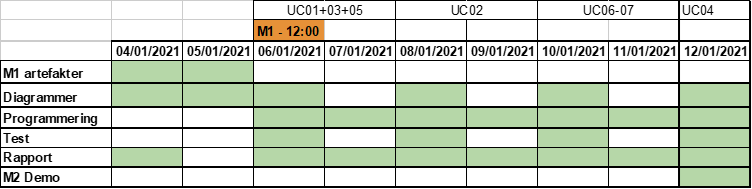
\includegraphics[width=14cm]{Report/figures/Projektplanlægning/Projektplanlægning_uge01.png}
    \caption{Projektplanlægning uge 1}
    \label{Projektplanlægning01}
\end{figure}

\begin{figure}[htp] %brug begin{figure} til alle figurer.
    \centering
    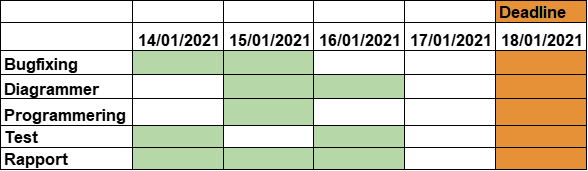
\includegraphics[width=14cm]{Report/figures/Projektplanlægning/Projektplanlægning_uge02.png}
    \caption{Projektplanlægning uge 2}
    \label{Projektplanlægning02}
\end{figure}

Det fremgår, at vi havde planlagt at være færdig med udviklingen af hele projektet den 16. Januar, hvorefter den sidste dag ville være hensat til uforudsete udfordringer eller fejl.

\end{flushleft}